\RequirePackage{lineno} 
\documentclass[a4paper,11pt,spanish]{article}

\usepackage[spanish]{babel}
\usepackage[utf8]{inputenc}
\usepackage{url}
\usepackage{graphicx} 
\usepackage{slashbox}
\usepackage{longtable}
\usepackage{multirow}
\usepackage{colortbl}
\usepackage{color}
\usepackage{lineno}
\usepackage{tikz}
 
\usepackage{gantt}
\setlength{\textheight}{24cm}
\textwidth=16.5cm
\topmargin=0cm
\oddsidemargin=0cm
\parindent=10mm

\begin{document}
%\linenumbers %activar nro de lineas
\pagestyle{empty}

\begin{center}

	\bigskip
	\bigskip
	
%	{\bf\Large Algoritmo para la detección de objetos planos aplicado a videos en un ambiente controlado.} \\
	{\bf\Large Método para detección y seguimiento de objetos con aplicaciones en Realidad Aumentada} \\
%	{\bf\Large Algoritmo para la detección de objetos planos en videos en un ambiente controlado.} \\

	\bigskip
	\bigskip

	\large Christian Nicolás Pfarher\\


  	\bigskip
  	\bigskip
	
	Punto de control N$^{\circ}$ 1 - Recopilación Bibliográfica \\	
	\bigskip
	
	Director\\
	\textit{Dr. Enrique Marcelo Albornoz}\\
	\bigskip
	Codirector\\
	\textit{Dr. César Martínez}\\
	
	\bigskip
	\bigskip
	\bigskip
	\bigskip
	\bigskip
	\bigskip
	\textit{\today}\\
	

	\vfill
	\begin{figure}[tbhp]
		\centerline{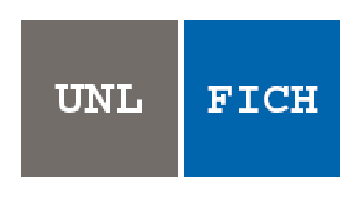
\includegraphics[scale=0.6]{img/fich_unl.eps}}
	\end{figure}
	
  	{Ingeniería Informática}\\
  	{Facultad de Ingeniería y Ciencias Hídricas}\\
    {UNIVERSIDAD NACIONAL DEL LITORAL}	
\end{center}

\bigskip
\bigskip

\newpage

\pagestyle{plain}

\section{Conceptos claves de Realidad Aumentada}
La Realidad Aumentada permite enriquecer la perspectiva sobre imponiendo objetos virtuales (2D o 3D) en el mundo real, con el objetivo de lograr persuadir al 
observador y haciéndole creer que el objeto virtual forma parte del ambiente real. De esta forma, se puede interpretar
la Realidad Aumentada, como una mezcla entre un mundo real y virtual tal como se visualiza en el diagrama Reality-Virtuality (RV) continuum diagram (Diagrama continuo de Realidad-Virtualidad) mostrado 
en la Fig. \ref{Reality-Virtuality Continuum}.
%================

%================

  \begin{figure}[tbhp]
    \centerline{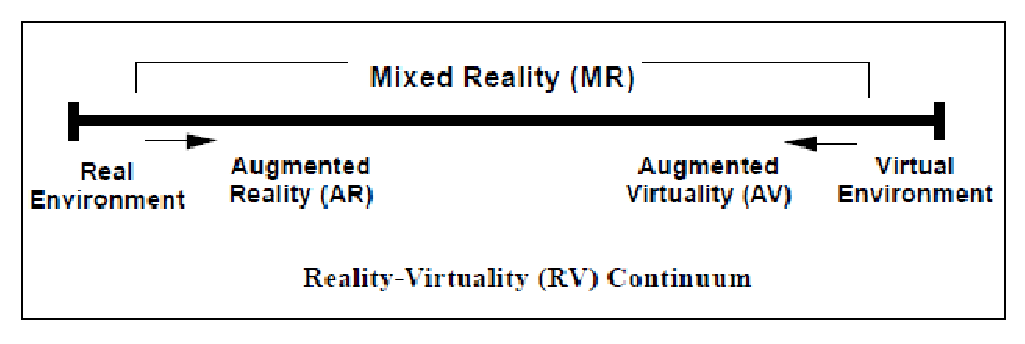
\includegraphics[scale=0.5]{img_ent1/reality_virtual.eps}}
    \caption{Reality-Virtuality Continuum (Diagrama continuo de Realidad-Virtualidad), Milgram, Takemura, Itsumi and Kishino \cite{Milgram94augmentedreality}}
    \label{Reality-Virtuality Continuum}
  \end{figure}

Algunos de los conceptos que se manejan en Realidad Aumentada son los siguientes:
\begin{description}
  \item [Reality View (Vista Real)] 
  Se refiere a la secuencia o stream de video producido por la cámara. La aplicación de Realidad Aumentada 
  captura imágenes desde esta secuencia de video, aumentándolas con objetos virtuales para crear una ``vista aumentada''. \cite{1320421}

  \item [Registration \& Tracking (Identificación y seguimiento)] 
  Describe los métodos disponibles para alinear un objeto virtual con un sistemas de coordenadas 
  en tres dimensiones en una vista real. En el seguimiento o Tracking, se pueden distinguir entre diferentes métodos: \textbf{location based tracking (seguimiento basado en localización)} y \textbf{optical tracking (seguimiento basado en visión)} o una combinación de ambos. \cite{conf/iswc/2007}, \cite{1320421}
  %================
  %================

  \item[Point of intereset-POI (Punto de interés)] 
  Es un elemento de información asociado con una ubicación geográfica (longitud, latitud, altura) o un patrón visual (marcador, tapa de libro, etc) 
  que se puede representar de alguna forma por la aplicación de Realidad Aumentada. \cite{1320421}, \cite{Azuma:2001:RAA:616073.618862}
  % El tipo de dato del punto de interés debe proporcionar una descripción de la localización o imagen de referencia utilizado en el seguimiento 
  % y el tipo de contenido que se dibujará (normalmente el contenido en si mismo (modelo 3d, imagen, etc) no es parte del 
  % punto de interés, pero un enlace al contenido se suministra en su lugar.
  %================
  %================
  \item [Virtual Object (Objeto Virtual)] 
  Es algún tipo de contenido digital que es dibujado por la aplicación de Realidad Aumentada y es sobre impuesto en la vista real. 
  Por lo general, incluye modelos 3D, imágenes 2D, iconos, textos, entre otros. \cite{conf/iswc/2007}, \cite{1320421}

  \item [Marker Based and Markerless AR (AR basados/no basados en marcadores)] 
  Cuando es utilizado el reconocimiento de imágenes para alinear un objeto virtual (optical tracking (seguimiento basado en visión)), hay una distinción entre sistemas:
  los que identifican un \textbf{marcador artificial} (código matricial 2D o diodo emisor de luz) colocado en un lugar determinado o sobre algún objeto del mundo real; los que utilizan la \textbf{detección de características naturales de los objetos}, para identificar objetos del mundo real inalterados (como tapas de libros, posters, etc.) los cuales no poseen marcas artificiales que asistan en el reconocimiento del objeto.
  En ambos casos, el objeto virtual 2D o 3D, aparece ``pegado'' al marcador o característica natural cuando se ve a través de la ventana gráfica de AR o Viewport. \cite{conf/iswc/2007}, \cite{1320421}

  \item [Location Based Tracking (Reconocimiento basados en localización)] 
  Se refiere al reconocimiento basado en información de geo-localización, obtenida a partir de dispositivos o sensores de localización. El término, es usado 
  para hacer una distinción entre sistemas que usan sensores de localización, en contraste con los que hacen tracking (seguimiento) del objeto usando técnicas de reconocimiento de imagen.
  El reconocimiento basado en localización, posee por lo general menos precisión que los métodos ópticos y es aplicado sobretodo en ambientes exteriores. \cite{1320421}, \cite{Azuma:2001:RAA:616073.618862}

  \item [Six Degrees of Freedom (6DoF) (Seis grados de libertad)] 
  Se refiere a la capacidad del sistema de seguimiento para mantener la alineación de un objeto del mundo real en un espacio tridimensional. Esto es, la capacidad de moverse hacia delante/atrás, arriba/abajo, izquierda/derecha (traslación en tres ejes perpendiculares), combinados con al rotación sobre
  tres ejes perpendiculares (guiñada, cabeceo, alabeo).

  Reconstruir la posición de la cámara con 6DoF es el objetivo más importante en AR, ya que de esta manera se determina la posición de la cámara y en consecuencia se obtiene la posibilidad de poder renderizar o dibujar los objetos virtuales en una perspectiva correcta. \cite{conf/iswc/2007}, \cite{1320421}, \cite{Azuma:2001:RAA:616073.618862}

\end{description}

\bigskip
\textbf{Referencias de la sección:
\cite{Milgram94augmentedreality}, %Paul Milgram et al., 1994 
\cite{1320421}, %Ben Butchart, 2011
\cite{conf/iswc/2007}, %Taehee Lee et al., 2007 6dof
\cite{Azuma:2001:RAA:616073.618862}, %Ronald Azuma et al., 2001
\cite{5739718}.% Ahyun Lee et al., 2010  sift lkt
}

\section{Puntos característicos y Descriptores}
La detección de puntos característicos (del inglés: keypoints o feature points) y descriptores de imágenes, es una característica ampliamente usada en problemas de reconocimiento de objetos, detección de imágenes, seguimiento visual, reconstrucción 3D entre otras aplicaciones. El objetivo recae en la idea de seleccionar ciertos puntos claves en una imagen, de forma que estos permitan distinguirla de otras sin la necesidad de tener que analizar la totalidad de la imagen.
Esta aproximación funciona correctamente, en la medida que se detecten la cantidad suficiente de puntos de interés que sean ``distinguibles'' y a su vez estables para que puedan ser nuevamente localizados en otra escena.

Existen diversos detectores de puntos característicos, descriptores y seguidores. Entre los algoritmos y métodos más destacados se pueden nombrar:
\begin{itemize}
 \item Harris Corner Detector (Detector de esquinas de Harris) \cite{citeulike:3484001}, \cite{citeulike:9456628}, \cite{TuytelaarsM07},
 \item FAST: Features From Accelerated Segment Test (Detección rápida de puntos característicos) \cite{citeulike:9456628},
 \item SIFT: Scale Invariant Feature Transform (Transformación de características invariante a la escala) \cite{citeulike:3484001}, \cite{citeulike:9456628}, \cite{TuytelaarsM07}, \cite{bb53077}, \cite{WagnerRMDS10}, \cite{conf/ismar/2004}, \cite{BouGar}, \cite{5739718}, 
 \item PCA-SIFT: Principal Components Analysis - Scale Invariant Feature Transform (Análisis de componentes principales - Transformación de características invariante a la escala) \cite{citeulike:3484001}, \cite{bb53077},
 \item SURF: Speeded Up Robust Features (Detector rápido de características robustas) \cite{citeulike:9456628}, \cite{Bay:2008:SRF}, \cite{TuytelaarsM07}, \cite{Bay:2008:SRF}, \cite{BouGar},
 \item KLT: Kanade–Lucas–Tomasi feature tracker (Seguidor de características Kanade-Lucas-Tomasi) \cite{citeulike:3484001}, \cite{TuytelaarsM07}, \cite{conf/ismar/2004}, \cite{5739718},
 \item L-K optical flow (Flujo óptico LK) \cite{citeulike:3484001}, \cite{citeulike:9456628}, \cite{conf/ismar/2004},
 \item SLAM: Simultaneous Localization And Mapping (Localización y Mapeado Simultáneos) \cite{Chen_markerlessaugmented}.
\end{itemize}

Otras técnicas ampliamente usadas en diferentes lineas de investigaciones junto a los métodos nombrados arriba son: K-D tree (árbol k-dimensional) \cite{citeulike:9456628} y RANSAC: RANdom SAmple Consensus (muestras aleatorias consensuadas) \cite{citeulike:9456628}.

\bigskip
\textbf{Referencias de la sección: \cite{citeulike:3484001}, %Gary Bradsky et al., 2008 
\cite{citeulike:9456628}, %Robert Laganière, 2011
\cite{Bay:2008:SRF},% Herbert Bay et al., 2008 surf
\cite{TuytelaarsM07}, %Tuytelaars et al., 2008 harris, surf, klt, sitf
\cite{bb53077}, %Krystian Mikolajczyk et al., 2005 sift, pca-sift
\cite{WagnerRMDS10}, %Daniel Wagner et al., 2010  sift, phony sift ferns
\cite{bb48614}, %Tsz-Wai Rachel Lo et al., 2009 sift
\cite{Chen_markerlessaugmented},% Ian Y-H Chen et al., 2008 slam OK
\cite{Bay:2008:SRF}, %Herbert Bay et al., 2007 surf
\cite{conf/ismar/2004}, %Iryna Skrypnyk et al., 2004 sift, klf
\cite{BouGar},% Óscar Boullosa García et al., 2011  sift surf
\cite{5739718}.% Ahyun Lee et al., 2010  sift lkt
}

\section{Operaciones morfológicas en imágenes}
Los filtros morfológicos son operadores que transforma una imagen de una forma predefinida (de acuerdo a la forma de la máscara aplicada). La interacción entre el filtro y los vecinos al píxel sobre el cuál se está aplicando el procesamiento, dan el resultado final de la transformación.

Técnicas como erosión, dilatación, detección de bordes y esquinas, umbralización, entre otras, son algunas clases de este tipo de operaciones que a veces son usadas como parte de un pre-procesamiento sobre las imágenes, para su posterior tratamiento.

\bigskip
\textbf{Referencias de la sección: \cite{citeulike:3484001}, %Gary Bradsky et al., 2008 
\cite{citeulike:9456628}, %Robert Laganière, 2011
\cite{bb1919}. %D. Conrad et al., 2010 
}

\section{Homografía y proyecciones}
Las imágenes generalmente son producidas usando una cámara, que captura la escena mediante la proyección de luz en un sensor a través de una lente. El hecho de que una imagen se forma a través de la proyección de una escena 3D en un plano 2D, impone la existencia de una importante relación entre la escena, la imagen y diferentes imágenes de la misma escena. La geometría proyectiva, es la herramienta usada para describir y caracterizar, en términos matemáticos, el proceso de formación de la imagen.

Algunos de los conceptos fundamentales en las relaciones proyectivas involucran temas tales como:
\begin{itemize} 
 \item el modelo pin-hole de la cámara \cite{citeulike:3484001}, \cite{citeulike:9456628},
 \item la calibración de la cámara que arroja como resultado los parámetros de distorsión y la matriz que la caracteriza \cite{citeulike:3484001}, \cite{citeulike:9456628}, \cite{Azuma:2001:RAA:616073.618862},
 \item Epipolos y lineas epipolares \cite{citeulike:3484001}, \cite{citeulike:9456628},
 \item Matriz fundamental \cite{citeulike:3484001}, \cite{citeulike:9456628}, \cite{Azuma:2001:RAA:616073.618862},
 \item Matching de imágenes usando RANSAC \cite{citeulike:3484001}, \cite{citeulike:9456628},
 \item Computo de homografía entre imágenes: una homografía, permite determinar la posición relativa de la cámara respecto a una escena. Es un mapeo uno a uno entre dos imágenes, el cual es definido por ocho parámetros. \cite{citeulike:3484001}, \cite{citeulike:9456628}, \cite{conf/icra/2010}.
\end{itemize}

\bigskip
\textbf{Referencias de la sección: \cite{citeulike:3484001}, %Gary Bradsky et al., 2008 
\cite{citeulike:9456628}, %Robert Laganière, 2011
\cite{conf/icra/2010}, %D. Conrad et al., 2010 
\cite{Azuma:2001:RAA:616073.618862}, %Ronald Azuma et al., 2001
\cite{5739718}. %44 Ahyun Lee et al., 2010
}
%%%%%%%%%%%%%%%%%%%%%%%%%%%%%%%%%%%%%%%%%%%%%%%%%%%%%%%%%%%%%%%%%%%%%%%%%%%%%%%%%%%%%%%%%%%%%%%%%%%%%%%%%%%
\newpage
\bibliographystyle{alpha}
\bibliography{bib1,bib4}

\end{document}
